\section{Viabilidad de dipolos y cuadrupolos para la simulación del haz}

Para poder ver el comportamiento de los campos de las dos configuraciones
contempladas, generados por dipolos y cuadrupolos, se crearon las siguientes
gráficas:

\begin{figure}[H] % Uso de [H] para mantener la figura en su posición
  \centering
  \begin{minipage}[b]{0.48\textwidth} % Ancho ajustado para que quepan dos imágenes
    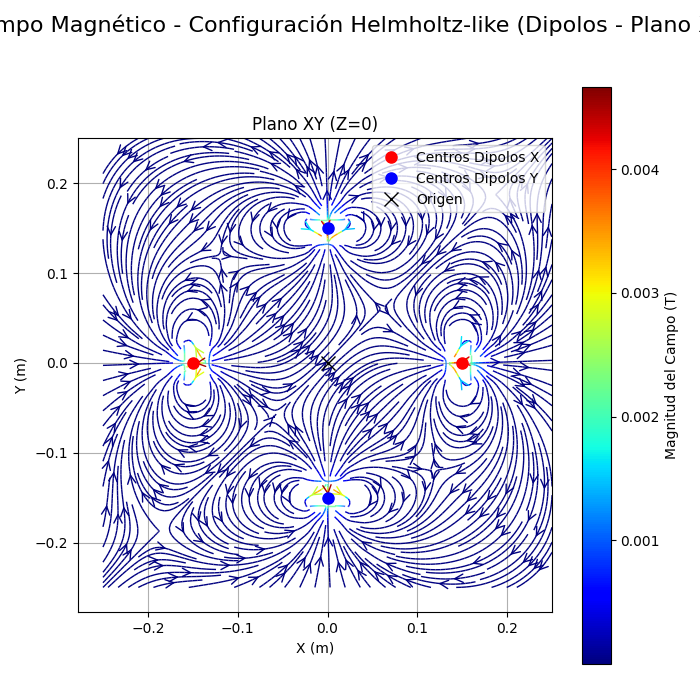
\includegraphics[width=\linewidth, trim={0cm 2cm 0cm 1cm}, clip]{Sections/Figures/helmholtz_dipoles_xy_field.png} % Valores de trim/clip de ejemplo
    \caption{Dipolos en Helmholtz.}
    \label{fig:helmholtz_dipoles_xy_field}
  \end{minipage}
  \hfill
  \begin{minipage}[b]{0.48\textwidth} % Ancho ajustado para que quepan dos imágenes
    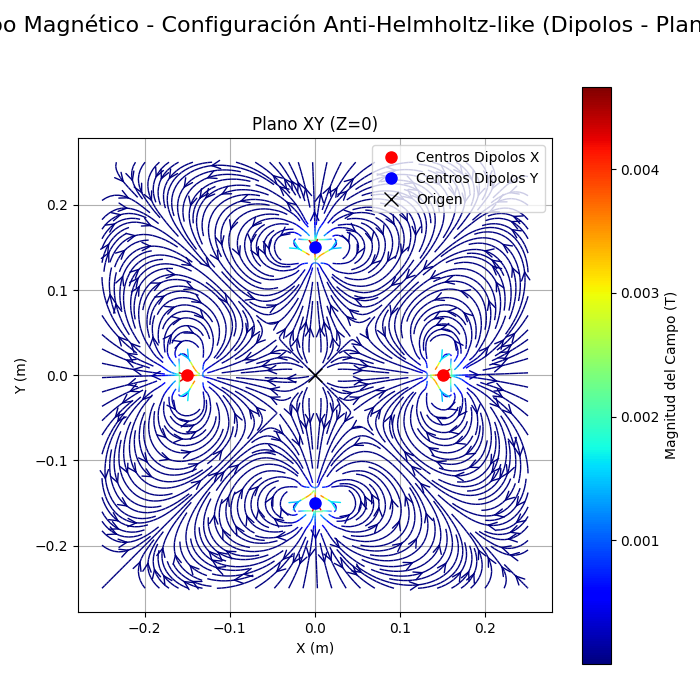
\includegraphics[width=\linewidth, trim={0cm 2cm 0cm 1cm}, clip]{Sections/Figures/antihelmholtz_dipoles_xy_field.png} % Valores de trim/clip de ejemplo
    \caption{Dipolos en Anti-Helmholtz.}
    \label{fig:antihelmholtz_dipoles_xy_field}
  \end{minipage}
  \caption{Morfología del campo magnético en el plano $x,y$ generado por dipolos en configuraciones Helmholtz y Anti-Helmholtz.}
  \label{fig:campos_dipolos}
\end{figure}

\begin{figure}[H] % Uso de [H] para mantener la figura en su posición
  \centering
  \begin{minipage}[b]{0.48\textwidth} % Ancho ajustado
    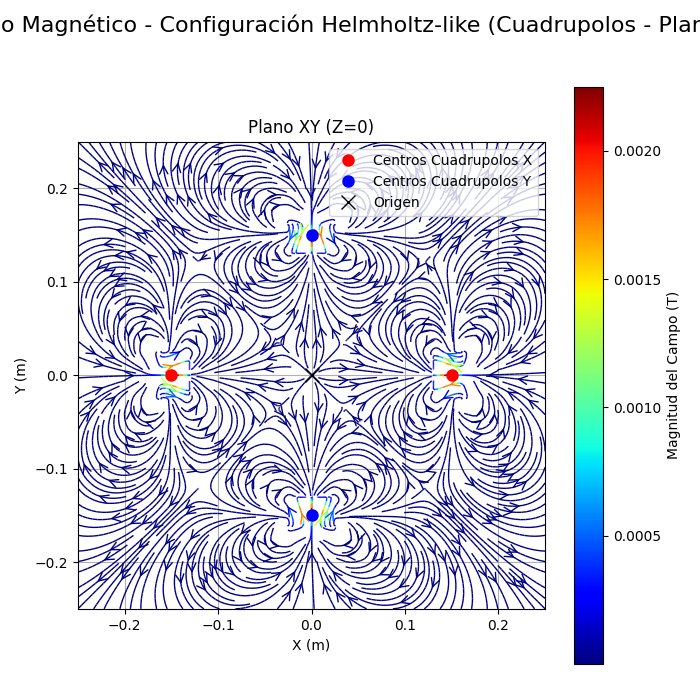
\includegraphics[width=\linewidth, trim={0cm 2cm 0cm 1cm}, clip]{Sections/Figures/helmholtz_quadrupoles_xy_field.png} % Valores de trim/clip de ejemplo
    \caption{Cuadrupolos en Helmholtz.}
    \label{fig:helmholtz_quadrupoles_xy_field}
  \end{minipage}
  \hfill
  \begin{minipage}[b]{0.48\textwidth} % Ancho ajustado
    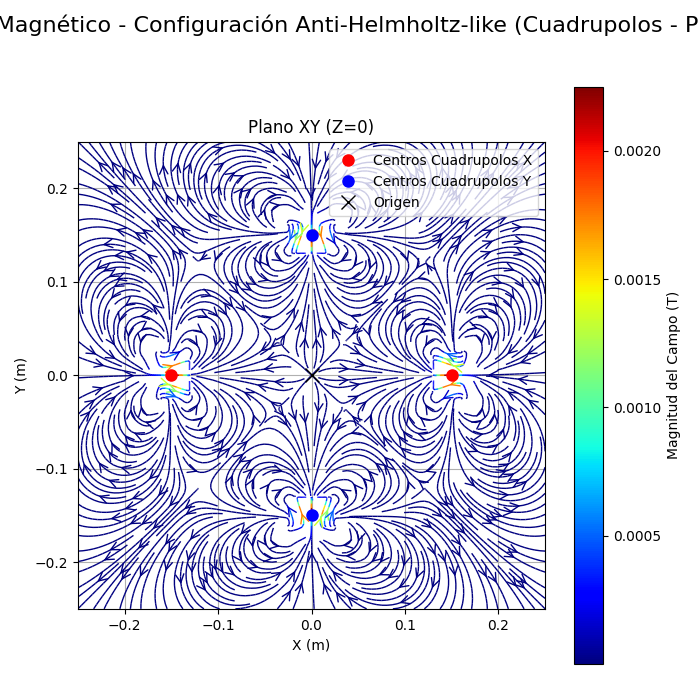
\includegraphics[width=\linewidth, trim={0cm 2cm 0cm 1cm}, clip]{Sections/Figures/antihelmholtz_quadrupoles_xy_field.png} % Valores de trim/clip de ejemplo
    \caption{Cuadrupolos en Anti-Helmholtz.}
    \label{fig:antihelmholtz_quadrupoles_xy_field}
  \end{minipage}
  \caption{Morfología del campo magnético en el plano $x,y$ generado por cuadrupolos en configuraciones Helmholtz y Anti-Helmholtz.}
  \label{fig:campos_cuadrupolos}
\end{figure}

Donde se planeaba fundamentalmente tomar el valor de la superposición de
estos campos y multiplicarlo por una expresión periódica que asimilara la
variación temporal de las corrientes de las bobinas, de la siguiente forma.

\begin{align*}
  \mathbf{B}_{\text{tot}}(\mathbf{r},t) &= \sin(\omega t + \gamma) \, \mathbf{B}_{\text{dipolo}}(\mathbf{r}) \\
  \mathbf{B}_{\text{tot}}(\mathbf{r},t) &= \sin(\omega t + \gamma) \, \mathbf{B}_{\text{cuadrupolo}}(\mathbf{r})
\end{align*}

Pero al ver el comportamiento de los campos generados en las imágenes, se llegó
a la conclusión de que la mejor forma de simular el sistema era directamente con
los campos generados por las bobinas.
